\documentclass[10pt]{article}

\usepackage[letterpaper,margin=0.88in]{geometry}
\usepackage[T1]{fontenc}
\usepackage{lmodern}
\usepackage{inconsolata}
\usepackage{microtype}
\usepackage{graphicx}
\usepackage{subcaption}
\usepackage{float}
\usepackage{booktabs}
\usepackage{tabularx}
\usepackage{array}
\usepackage{amsmath}
\usepackage{siunitx}
\usepackage[labelfont=bf,font=small]{caption}
\usepackage{enumitem}
\usepackage[dvipsnames]{xcolor}
\usepackage[hidelinks]{hyperref}

\newcommand{\projectname}{CreditSense: Loan Risk Assessment Challenge}
\newcommand{\teamname}{Johnny-Izhak-Kyriakos}
\newcommand{\studentnames}{Matvei, Izhak, Kyriakos}
\newcommand{\kaggleuser}{JohnnyC0rp}
\newcommand{\publicscore}{0.8495}
\newcommand{\localbestscore}{0.8576}


\setlength{\parindent}{0pt}
\setlength{\parskip}{0.35em}
\setlist[itemize]{leftmargin=1.25em,itemsep=0.2em,topsep=0.2em}
\setlist[enumerate]{leftmargin=1.25em,itemsep=0.2em,topsep=0.2em}

\pagestyle{plain}

\begin{document}

\begin{titlepage}
    \thispagestyle{empty}
    \begin{center}
        \vspace*{\fill}
        {\large MBZUAI \par}
        \vspace{0.55cm}
        {\large AI1215 --- Introduction to Machine Learning \par}
        \vspace{1.5cm}
        {\Huge\bfseries \projectname \par}
        \vspace{0.45cm}
        {\Large Final Project Report \par}
        \vspace{1.6cm}
        \rule{0.72\linewidth}{0.9pt}
        \vspace{0.85cm}

        \begin{tabular}{rl}
            Team name: & \teamname \\
            Students: & \studentnames \\
            Kaggle username: & \kaggleuser \\
            Final submission family: & \texttt{meta\_overnight} \\
            Date: & April 2026 \\
        \end{tabular}

        \vspace{0.9cm}
        \rule{0.72\linewidth}{0.5pt}
        \vspace*{\fill}
    \end{center}
\end{titlepage}

This report summarizes the final submitted pipeline for the CreditSense challenge. The task combines a five-class classification problem with a bounded regression problem, and Kaggle scores each submission by averaging classification accuracy and regression \(R^2\). Our development therefore focused on changes that improved both targets at the same time, while keeping the final solution reproducible from the saved branch artifacts and the final implementation.

\section{Data Exploration and Preprocessing}

The training set contains 35{,}000 applicants, 55 predictors, and two targets: \texttt{RiskTier} for Task A and \texttt{InterestRate} for Task B. Because the public score is the mean of accuracy and \(R^2\), every design choice was checked against both targets on the same fixed validation split. This was important in practice: a change that helped classification but damaged the rate model was usually not worth keeping.

The first useful observation was that the dataset was not dominated by class imbalance. Figure~\ref{fig:eda-summary} shows that all five risk tiers are well represented, so we did not use class reweighting or resampling. The more serious issue was structured missingness. The columns with the highest missing rates were \texttt{StudentLoanOutstandingBalance} (59.98\%), \texttt{CollateralType} (55.06\%), \texttt{CollateralValue} (54.64\%), \texttt{MortgageOutstandingBalance} (45.18\%), and \texttt{PropertyValue} (45.05\%). Those gaps were not random; they reflected borrower state.

\begin{figure}[H]
    \centering
    \begin{subfigure}[t]{0.48\linewidth}
        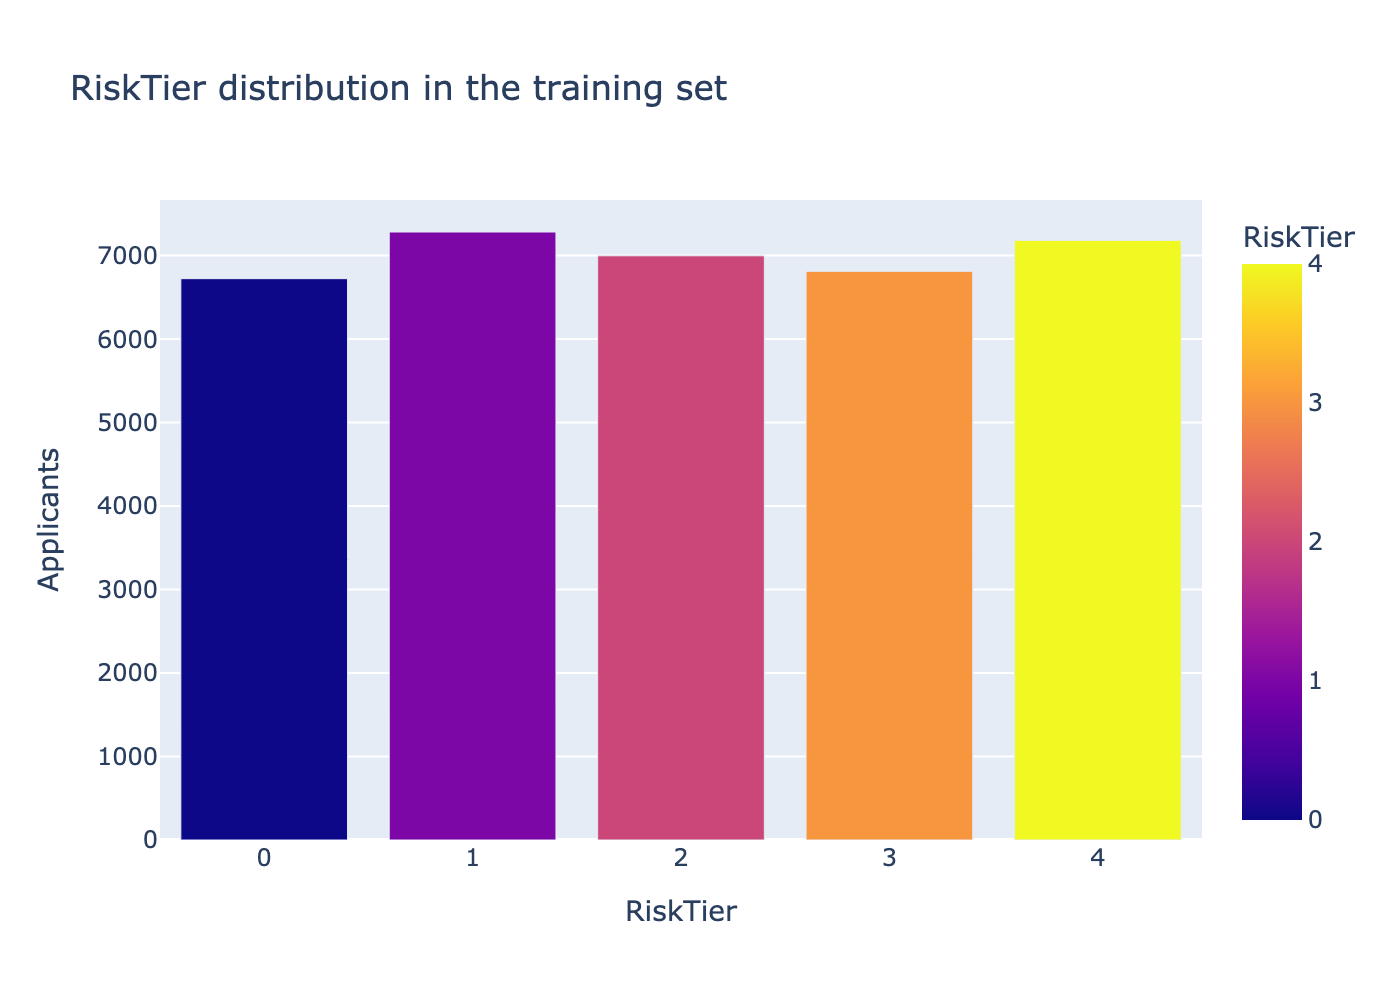
\includegraphics[width=\linewidth]{figures/class_distribution.png}
        \caption{Risk tiers are reasonably balanced.}
    \end{subfigure}
    \hfill
    \begin{subfigure}[t]{0.48\linewidth}
        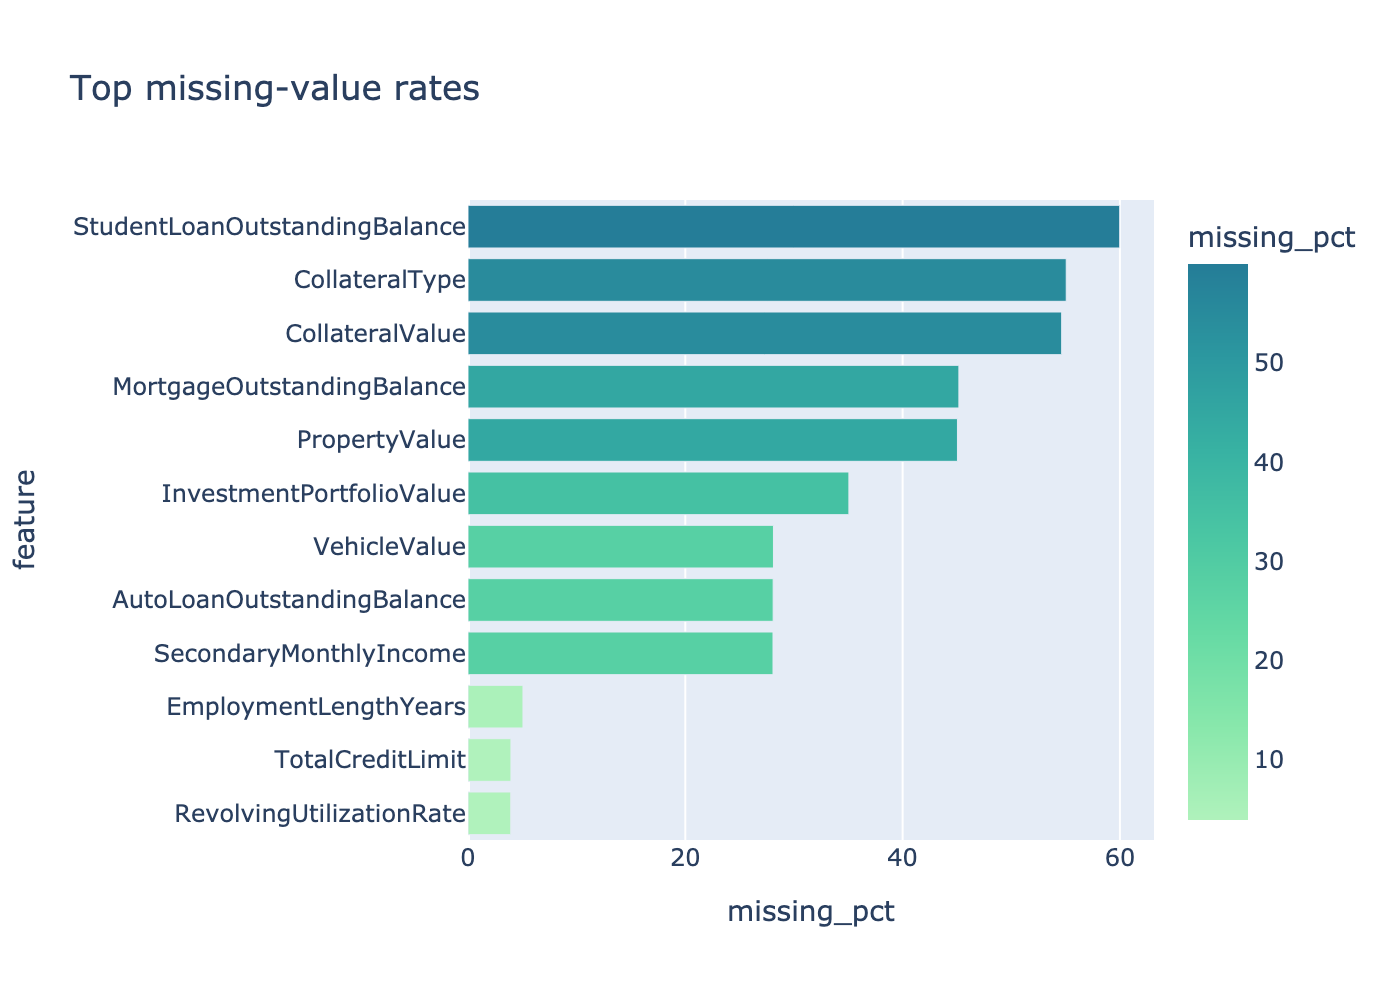
\includegraphics[width=\linewidth]{figures/missingness_overview.png}
        \caption{Missingness is concentrated in meaningful financial columns.}
    \end{subfigure}
    \caption{The early data check was reassuring in one way and tricky in another: class balance was fine, but missing values clearly carried signal.}
    \label{fig:eda-summary}
\end{figure}

That point becomes clearer once the missing columns are conditioned on context. In Figure~\ref{fig:context-corr}, \texttt{PropertyValue} and \texttt{MortgageOutstandingBalance} are missing for about 80\% of renters and applicants living with family, but only for about 16--17\% of owners or mortgage holders. Student-loan balances show a similar pattern by age: they are absent for the entire oldest age bucket and present much more often for younger borrowers. We therefore treated missingness as a feature to explain, not noise to erase.

\begin{figure}[H]
    \centering
    \begin{subfigure}[t]{0.48\linewidth}
        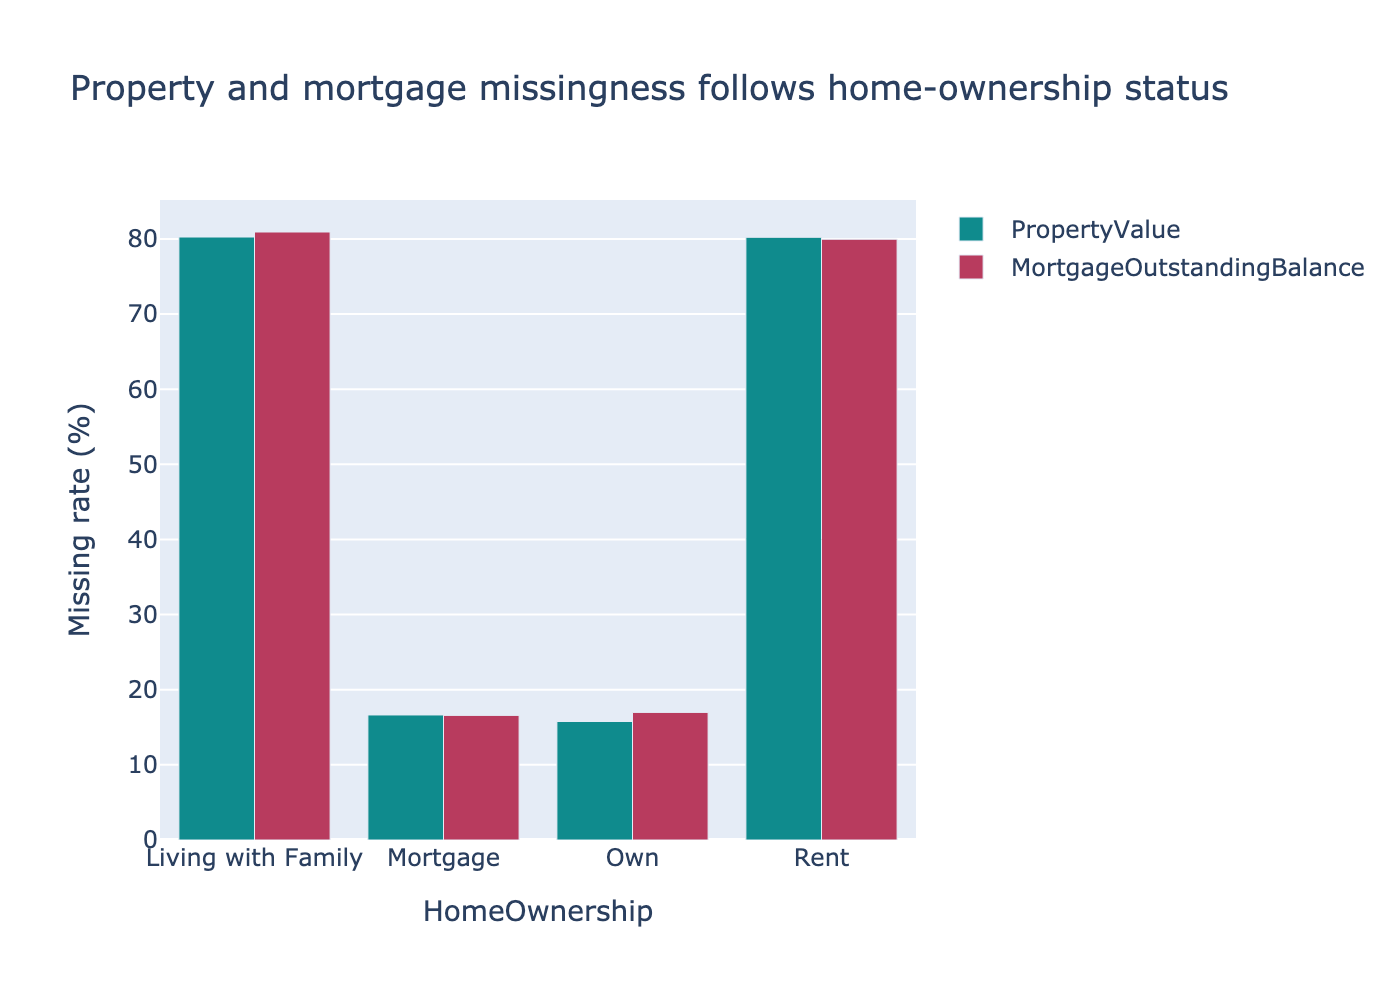
\includegraphics[width=\linewidth]{figures/semantic_missingness_context.png}
        \caption{Property and mortgage blanks are tightly linked to home-ownership status.}
    \end{subfigure}
    \hfill
    \begin{subfigure}[t]{0.48\linewidth}
        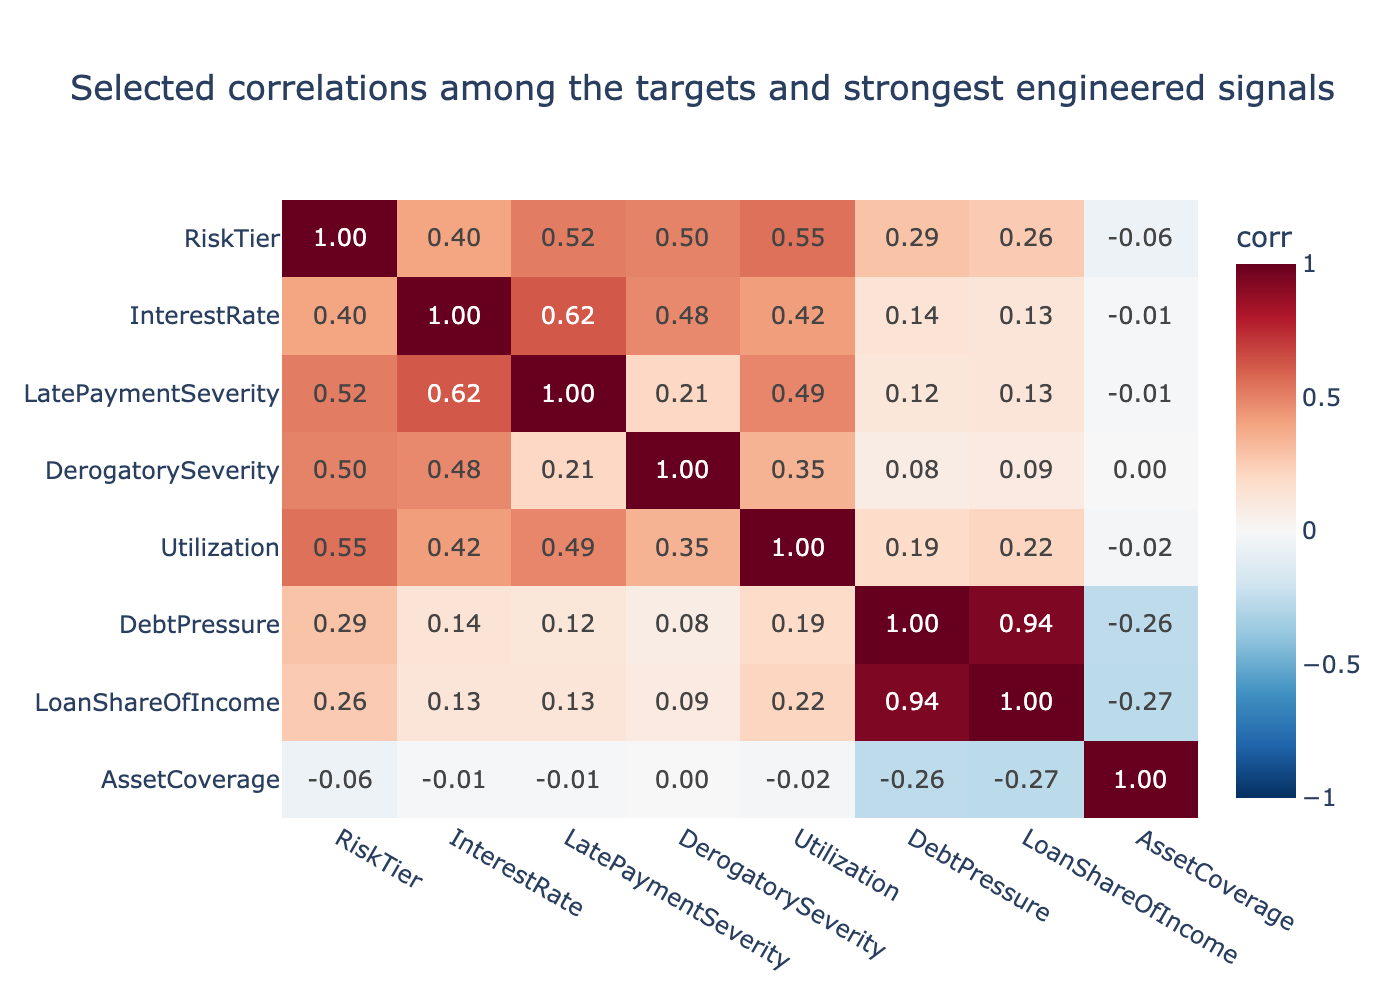
\includegraphics[width=\linewidth]{figures/correlation_focus.png}
        \caption{Delinquency and utilization features align most strongly with both targets.}
    \end{subfigure}
    \caption{Two findings shaped the rest of the pipeline: missing values were contextual, and the strongest raw relationships were concentrated in delinquency and utilization signals.}
    \label{fig:context-corr}
\end{figure}

The second useful observation was that the two targets overlap, but not perfectly. The mean offered APR rises from 6.01\% in tier 0 to 11.55\% in tier 4, yet there is still visible overlap across the lower four classes. This is why the regression problem could not simply be treated as a deterministic mapping from the class label. The correlation heatmap in Figure~\ref{fig:context-corr} makes the same point from another angle: \texttt{RevolvingUtilizationRate}, \texttt{LatePaymentSeverity}, and \texttt{DerogatorySeverity} correlate most strongly with both targets, while affordability and coverage features are weaker but still complementary.

Preprocessing was intentionally conservative:
\begin{itemize}
    \item numeric columns were median-filled only after explicit missingness indicators were created;
    \item categorical columns were preserved as strings for CatBoost, while the shared matrix used stable ordinal encoding and simple frequency features;
    \item no resampling was applied because the class histogram was already balanced enough;
    \item one fixed stratified split with seed 42 was reused for branch comparison and feature screening.
\end{itemize}

These choices kept the raw borrower structure intact. In particular, the preprocessing stage did not try to smooth away financial asymmetries that later became useful engineered features.

\section{Feature Engineering}

Most of the score jump came from feature work, not from swapping one model for another. The raw columns were already useful, but they hid the borrower story. We got much better results once we started writing features that sounded like lending questions instead of spreadsheet formulas.

\begin{table}[H]
    \centering
    \small
    \begin{tabularx}{\linewidth}{@{} p{0.22\linewidth} p{0.34\linewidth} X @{}}
        \toprule
        Feature family & Examples & Why it stayed in the final public pipeline \\
        \midrule
        Affordability ratios & loan share of income, monthly payment share, asset coverage & These features turned raw balances into simple stress indicators and helped both targets. \\
        Delinquency features & weighted late-payment counts, severity over history length, utilization interactions & They were consistently strong for \texttt{RiskTier} and also improved rate prediction. \\
        Derogatory burden & charge-off, collection, bankruptcy, and public-record aggregates & A compact way to summarize past damage without relying on a single raw field. \\
        Semantic missingness & renter-without-property, owner-without-mortgage, no-collateral flags & These features captured why a field was blank, which was often more useful than the filled value itself. \\
        Controlled interactions & selected pairwise products between stress and balance features & A small interaction set helped the tree models find sharper non-linear boundaries. \\
        \bottomrule
    \end{tabularx}
    \caption{Feature groups that mattered enough to survive into the best public lane.}
    \label{tab:feature-families}
\end{table}

Figure~\ref{fig:feature-signal} shows the same pattern from another angle. The two targets overlap, but they do not rank features in exactly the same way. Delinquency and utilization features dominate the classification side, while affordability and balance-sheet coverage matter a bit more for the rate regression.

\begin{figure}[H]
    \centering
    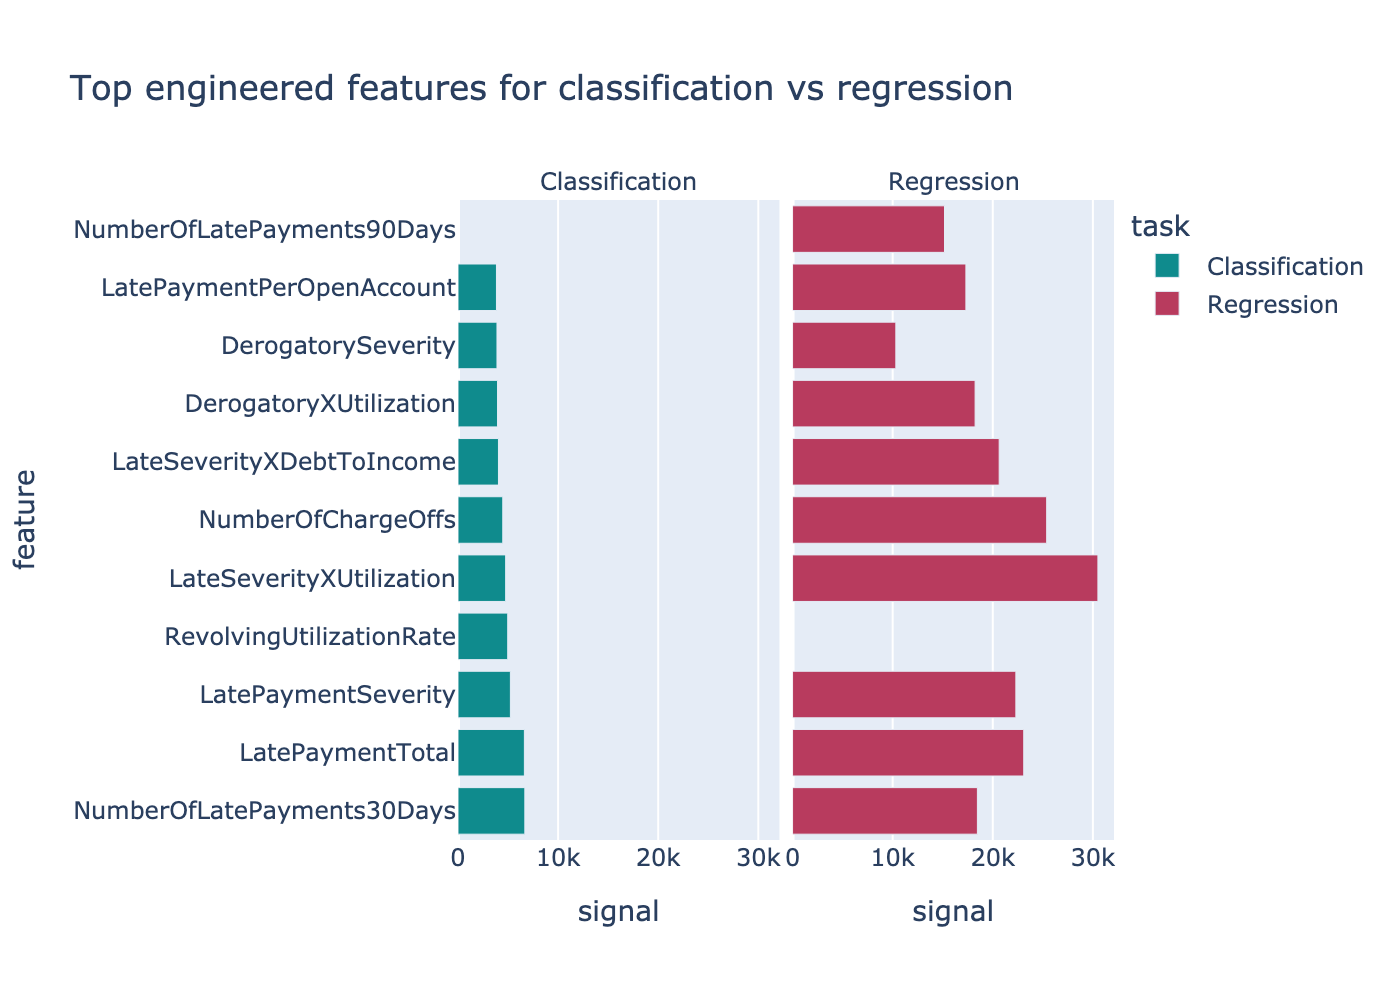
\includegraphics[width=\linewidth]{figures/feature_signal_comparison.png}
    \caption{The strongest engineered features overlap across targets, but the ordering is not identical.}
    \label{fig:feature-signal}
\end{figure}

We also tracked how the score changed when major feature ideas were added. The important pattern is not that every extra trick helped, but that the first few feature families changed the game while later additions gave smaller and more selective gains. The overall project progression later in the report follows the same logic.

\section{Model Selection \& Final Pipeline}

After the feature set settled down, the model story became much cleaner. Single models were good enough to guide the search, but the best public path came from letting several branch families vote in different ways:
\begin{enumerate}
    \item XGBoost on the engineered numeric matrix.
    \item LightGBM on the same processed frame.
    \item CatBoost on the mixed feature table with categorical columns preserved.
    \item ExtraTrees as a strong but simpler diversity branch.
    \item An MPS neural branch to add a different error profile.
\end{enumerate}

Instead of freezing mysterious blend weights inside the report code, the public repo now reads the original tuned branch configurations from saved overnight artifacts and fits the blend/meta combiner openly in code. That is closer to how the actual project worked and much easier to explain.

\begin{table}[H]
    \centering
    \small
    \begin{tabular}{@{} l c c c @{}}
        \toprule
        Model & Accuracy & \(R^2\) & Combined \\
        \midrule
        \texttt{meta\_overnight} & 0.8477 & 0.8513 & \textbf{0.8495} \\
        \texttt{blend\_overnight} & 0.8424 & 0.8485 & 0.8455 \\
        \texttt{target\_stats\_blend} & 0.8563 & 0.8552 & 0.8557 \\
        \texttt{mlp\_meta\_stack\_v1} & 0.8587 & 0.8556 & 0.8572 \\
        \texttt{mlp\_weighted\_blend\_v1} & 0.8600 & 0.8553 & \textbf{0.8576} \\
        \bottomrule
    \end{tabular}
    \caption{Representative validation checkpoints from the project.}
    \label{tab:model-table}
\end{table}

\begin{figure}[H]
    \centering
    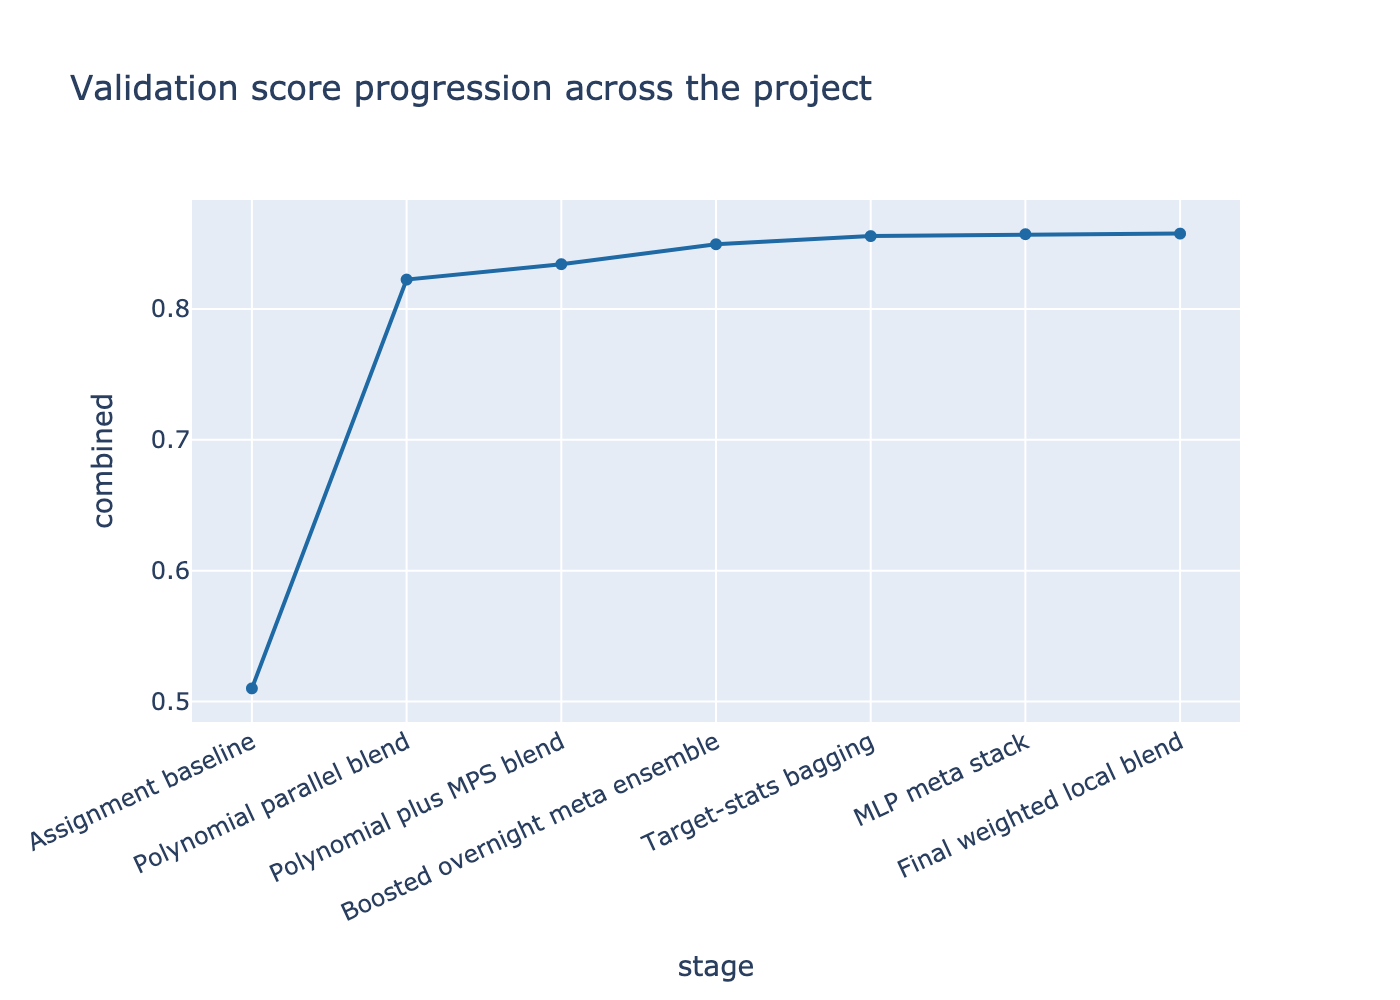
\includegraphics[width=0.86\linewidth]{figures/stage_progress.png}
    \caption{The project kept improving after the public-best lane, but those later gains came from heavier local-only combinations rather than a cleaner public submission path.}
    \label{fig:stage-progress}
\end{figure}

The final choice was mostly a trade-off between clarity and squeezing out the last few thousandths. We did reach a stronger local score later, but that route was harder to present cleanly and harder to justify as the main public notebook. For the repo and the report, \texttt{meta\_overnight} is the right landing point: strong score, readable branch structure, and a direct path from raw CSVs to a final submission file.


\end{document}
